%%%%%%%%%%%%%%%%%%%%%%%%%%%%%%%%%%%%%%%%%%%%%%%%%%%
%% LaTeX book template                           %%
%% Author:  Amber Jain (http://amberj.devio.us/) %%
%% License: ISC license                          %%
%%%%%%%%%%%%%%%%%%%%%%%%%%%%%%%%%%%%%%%%%%%%%%%%%%%

\documentclass[a4paper,11pt]{report}
\usepackage[T1]{fontenc}
\usepackage[utf8]{inputenc}
\usepackage{lmodern}
%%%%%%%%%%%%%%%%%%%%%%%%%%%%%%%%%%%%%%%%%%%%%%%%%%%%%%%%%
% Source: http://en.wikibooks.org/wiki/LaTeX/Hyperlinks %
%%%%%%%%%%%%%%%%%%%%%%%%%%%%%%%%%%%%%%%%%%%%%%%%%%%%%%%%%
\usepackage{hyperref}
\usepackage{graphicx}
\usepackage[english]{babel}

\usepackage{listings}
\usepackage{xcolor}

\usepackage[nottoc]{tocbibind}
\usepackage{bibentry}


\definecolor{codegreen}{rgb}{0,0.6,0}
\definecolor{codegray}{rgb}{0.5,0.5,0.5}
\definecolor{codepurple}{rgb}{0.58,0,0.82}
\definecolor{backcolour}{rgb}{0.95,0.95,0.92}



\newcommand\blfootnote[1]{%
	\begingroup
	\renewcommand\thefootnote{}\footnote{#1}%
	\addtocounter{footnote}{-1}%
	\endgroup
}


\graphicspath{ {./images/} }


%%%%%%%%%%%%%%%%%%%%%%%%%%%%%%%%%%%%%%%%%%%%%%%%
% Chapter quote at the start of chapter        %
% Source: http://tex.stackexchange.com/a/53380 %
%%%%%%%%%%%%%%%%%%%%%%%%%%%%%%%%%%%%%%%%%%%%%%%%
\makeatletter
\renewcommand{\@chapapp}{}% Not necessary...
\newenvironment{chapquote}[2][2em]
  {\setlength{\@tempdima}{#1}%
   \def\chapquote@author{#2}%
   \parshape 1 \@tempdima \dimexpr\textwidth-2\@tempdima\relax%
   \itshape}
  {\par\normalfont\hfill--\ \chapquote@author\hspace*{\@tempdima}\par\bigskip}
\makeatother

%%%%%%%%%%%%%%%%%%%%%%%%%%%%%%%%%%%%%%%%%%%%%%%%%%%
% First page of book which contains 'stuff' like: %
%  - Book title, subtitle                         %
%  - Book author name                             %
%%%%%%%%%%%%%%%%%%%%%%%%%%%%%%%%%%%%%%%%%%%%%%%%%%%

% Book's title and subtitle
\title{\Huge \textbf{CSE 6708 - Semantic Web} \\
	 \huge Assignment 2 \\
	 \normalsize Report on Paper Presentation \\
	 \normalsize \textbf{Paper Name} Source Code Plagiarism Detection Method Using Protégé Built Ontologies
}
% Author
\author{\textsc{Samidhya Sarker} \\ Student No. 1018052049 \\ Group-2}



\begin{document}

%\frontmatter
\maketitle

%%%%%%%%%%%%%%%%%%%%%%%%%%%%%%%%%%%%%%%%%%%%%%%%%%%%%%%%%%%%%%%%%%%%%%%%
% Auto-generated table of contents, list of figures and list of tables %
%%%%%%%%%%%%%%%%%%%%%%%%%%%%%%%%%%%%%%%%%%%%%%%%%%%%%%%%%%%%%%%%%%%%%%%%
\tableofcontents
\listoffigures
%\lstlistoflistings
%\listoftables

%\mainmatter

%%%%%%%%%%%
% Preface %
%%%%%%%%%%%

\chapter{Paper Summery}

Extending the conclusion started in Assignment 1\footnote{\url{https://semantic-web.netlify.com/report/report.pdf}}, 
I can say that the paper is an excellent scientific article if we think about how to present only the relevant information
without any clutter. \\\\Quoting from assignment 1\footnotemark[1], several tasks have been done:
\begin{enumerate}
	\item Creating ontologies from source code manually by hand using protege.
	\item Executing SPARQL queries on ontologies and compare the metrics.
	\item Creating topic maps using Protege OntoGraf plugin.
\end{enumerate} 
The paper serves an excellent purpose of being a showcase of semantic web technologies. Also, It addresses an important issue in CS education. Then again, I can think of several shortcomings regarding this fine 
piece of scientific literature.  \\

For instance the authors do not give a specific implementation, only a prototype which only performs manual
owl ontology extraction and doing SPARQL query. But specific implementaions of source code parsing for source
code navigation exists\cite{atzeni2017codeontology}\cite{zimmer2004tuna}. For example, github has already a \textit{navigate}\footnote{\url{https://help.github.com/en/articles/navigating-code-on-github}} feature which uses
the open source sibrary \textit{semantic}\footnote{\url{https://github.com/github/semantic}} to parse, analyze and compare source code. Incidentally, \textit{semantic} is written in \textit{Haskell} and I think functional programming 
languages with strong static typing is most appropriate for this task. Powerful transpilers (for example: Corrode \footnote{\url{https://github.com/jameysharp/corrode}}) have been written using \textit{Haskell} and the main
goal of using \textit{Racket}\footnote{\url{https://racket-lang.org/}} is to write domain specific languages. \\

Another thing I can think of is that, the authors are only retrieving information from lexical analysis.
Due to compiler optimization, we can say that, the source code programmer writes and the end result of 
a compiler toolchain has many leaps and bounds. So, a plagiarizer may escape scrutiny by changing unnecessary lexical 
things in source code or by subtle structural changes. On the contrary, there is a great chance of false-positives if we do not cross check the results of SPARQL query and topic maps with visual checking.  \\

The main promising application of semantic web technologies is to create
a knowledge base aiding information sciences. So, the main application of 
semantic technologies should be the analytics, navigation and information 
gathering from source codes. Although semantic indexing can aid traditional applications.\\

A by-product of semantic plagiarism detection will be creating a intelligent code search engine. There are 
a autocomplete plugin named \textit{Kite}\footnote{\url{https://kite.com/}} which uses machine learning to
search for code snippet or documentation. There are other tools like \textit{Sourcegraph}\footnote{\url{https://about.sourcegraph.com/}} and \textit{Bing C\# Code Search}\footnote{\url{https://codesnippet.research.microsoft.com/}} which might use fuzzy matching and other graph search
algorithms. Using semantic indexing will surely augment their search functions and provide multiplications of 
productivity. \\

In the case of plagiarization detections, Powerful utilites like \textbf{JPlag}\footnote{\url{https://jplag.ipd.kit.edu/}}, \textbf{MOSS}(Measure Of Software Similarity)\footnote{\url{http://theory.stanford.edu/~aiken/moss/}} etc. already exists.
As they are open source products, We may try to use these and add semantic elements in them rather than implementing a
new system from scratch.


\chapter{Analysis of References present in Given Paper}

\section{List of References}

\begin{enumerate}
    \item M. K. Shenoy, K. C. Shet and U. D.  Acharya. (2012, May). Semantic Plagiarism Detection System Using Ontology Mapping.  Advanced Computing: An International Journal 3(3). \footnote{\url{http://airccse.org/journal/acij/papers/0512 acij06.pdf}} \label{listref1}
    
    \item The Protégé Ontology Editor and Knowledge Acquisition System. \footnote{\url{http://protege.stanford.edu/}} (2013, July 1).  \label{listref2}
    
    \item T. Bray, J. Paoli, C. M. Sperberg-McQueen, E. Maler and F. Yergeau.  (2004, February 4). Extensible Markup Language (XML) 1.0.  W3C Recommendation . Third Edition.
    \footnote{\url{http://www.w3.org/TR/2004/REC-xml20040204/}} \label{listref3}
    
    \item F. Manola and E. Miller (2004, February 10). RDF Primer. W3C Recommendation. \footnote{\url{http://www.w3.org/TR/2004/REC-rdfprimer-20040210/}} \label{listref4}
    
    \item S. Harris, A. Seaborne. (2013, March 21).  SPARQL 1.1 Query Language. W3C Recommendation. Available: \footnote{\url{http://www.w3.org/TR/2013/RECsparql11-query-20130321/}} \label{listref5}
    
    \item J. Bao, D. Calvanese, B. C. Grau, et al.  (2012, December 11). OWL 2 Web Ontology Language.  W3C Recommendation.  Second Edition. \footnote{\url{http://www.w3.org/TR/owl2-overview/}} \label{listref6}
    
    \item E Akin, Object Oriented Programming, Houston: Rice University Publishing House, 2001, pp. 33-34.\label{listref7}
    
    \item S. Kara, O. Alan and O. Sabuncu, “An ontology-based retrieval system using semantic indexing”, Information Systems, vol. 37, no. 4, pp. 294–305, June 2012. \label{listref8}
    
    \item Pseudocode Standards, California Polytechnic State University Website. 
    \footnote{\url{http://users.csc.calpoly.edu/~jdalbey/SW E/pdl\_std.html (2013, July 1)}}\label{listref9}
    
    \item C. Liu, H. Wang, Y. Yu and L. Xu, “Towards Efficient SPARQL Query Processing on RDF Data”, Tsinghua Science \& Technology, vol. 15, no. 6, pp.  613–622, December 2010.\label{listref10}
    
    \item I. Ivan and C. Boja, Metode Statistice in analiza software. Bucharest: ASE Publishing House, 2004, pp. 218-224.  Informatica Economică vol. 17, no. 3/2013\label{listref11}
    
    \item S. Russel and P. Norving, Artificial Intelligence: A Modern Approach (2nd edition). New Jersey: Pearson Education Inc., 2003, pp. 350-352.\label{listref12}
    
    \item P. Durusau, S. Newcomb and R. Barta (2007, November). Topic Maps Reference Model. International Organization for Standardization. \footnote{\url{http://www.isotopicmaps.org/TMRM/TM RM-7.0/tmrm7.pdf}}\label{listref13}
    
    \item D. Newman, T. Baldwin, L. Cavedon and E. Huang, “Visualizing search results and document collections using topic maps”, Web Semantics: Science, Services and Agents on the World Wide Web, vol. 8, no. 2-3, pp 169–175, July 2010.\label{listref14}
    
    \item A. Hatzigaidas, A. Papastergiou, G.  Tryfon and D. Maritsa, “Topic Map Existing Tools: A Brief Review”, in Proc.  The International Conference on Theory and Applications of Mathematics and Informatics, Thessaloniki, Greece, 2004, pp 185-201  \label{listref15}
\end{enumerate}

\section{Classification of Given Citation}

\begin{itemize}
	\item Reference \ref{listref1} is a paper published in an international Journal.
	
	\item Reference \ref{listref2} is the homepage of Protege editor.
	
	\item Reference \ref{listref3} is World Wide Web Consortium (W3C) recommendation of XML. 

	\item Reference \ref{listref4} is World Wide Web Consortium (W3C) primer for RDF.

	\item Reference \ref{listref5} is World Wide Web Consortium (W3C) recommendation for SPARQL.
	
	\item Reference \ref{listref6} is  Wide Web Consortium (W3C) recommendation for OWL. 

	\item Reference \ref{listref7} is a book on OOP.
	 
	\item Reference \ref{listref8} is a Masters thesis from Middle East University (Turkey) on semantic indexing.
	
	\item Reference \ref{listref9} is a dead link to a standard on pseudocode writing. Currently can be found on scribd \footnote{\url{https://www.scribd.com/document/47856615/PSEUDOCODE-STANDARD}}.
	
	\item Reference \ref{listref10} is an IEEE paper on SPARQL Query processing.

	\item Reference \ref{listref11} is an book on Statistical methods in software analysis written in Romanian. 
	
	\item Reference \ref{listref12} is the most widespread book on AI. 
	
	\item Reference \ref{listref13} is the ISO reference model for topic maps. 
	
	\item Reference \ref{listref14} is a article from Elsevier on how to visualize data using topic maps.
	
	\item Reference \ref{listref15} is an paper published in an international conference on tools required to implement topic maps. 
	
\end{itemize}

\subsection{Comment}

As we can see that references 3-6, 13 are specifications from W3C, ISO. Reference 2 is a website.
And References 11, 12 are excerpts from books. So, we shall analyze refences 1, 8, 10, 14, 15.

\section{Reference 1: Semantic Plagiarism Detection System Using Ontology Mapping}

In this paper, the authors discuss the applications of using Semantic web ontologies to detect 
plagiarism in text documents. The proposal is to train an ontology learner by feeding an ontology 
mapping algorithm (a) Main copies and (b) Probable plagiarizations. \\

The authors also experimented with a prototype TAO (Transitioning Applications to Ontologies) project but the implementation details are not given.

\begin{figure}[]
	\label{ref_1_arch}
	\centering 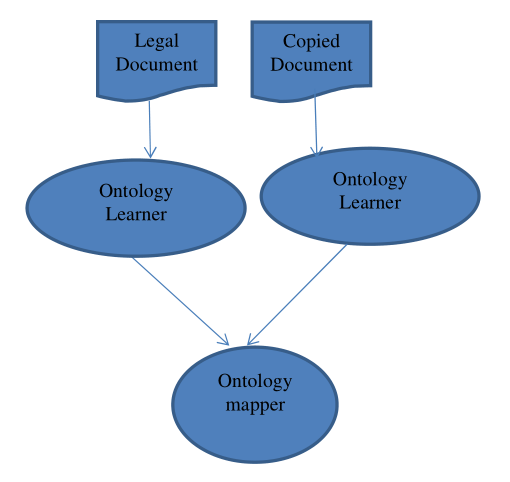
\includegraphics[scale=0.5]{ref_1_arch.png}
	\caption{Architecture of the proposed detection system.}
\end{figure}

\break

\section{Reference 8: An ontology-based retrieval system using semantic indexing}

This Masters thesis, can be divided into three parts. In chapter 2, Background information,
the authors discuss general information science with an emphasis on information retrieval (IR).
They also discuss optimizing the information retrieval or searching process implementing indexing,
ranking etc. They also discusss evaluation metrices. Finally the concept of Semantic Web is 
introduced and the application to improve IR is discussed. \\

In chapter 3, various approaches including traditional, semantic approaches are discussed. 
The authors discuss semantic indexing and their proposed models. \\

In chapter 4, the authors conceptualize their own semantic retrieval process. 

\begin{figure}[h]
	\label{ref_8_design}
	\centering 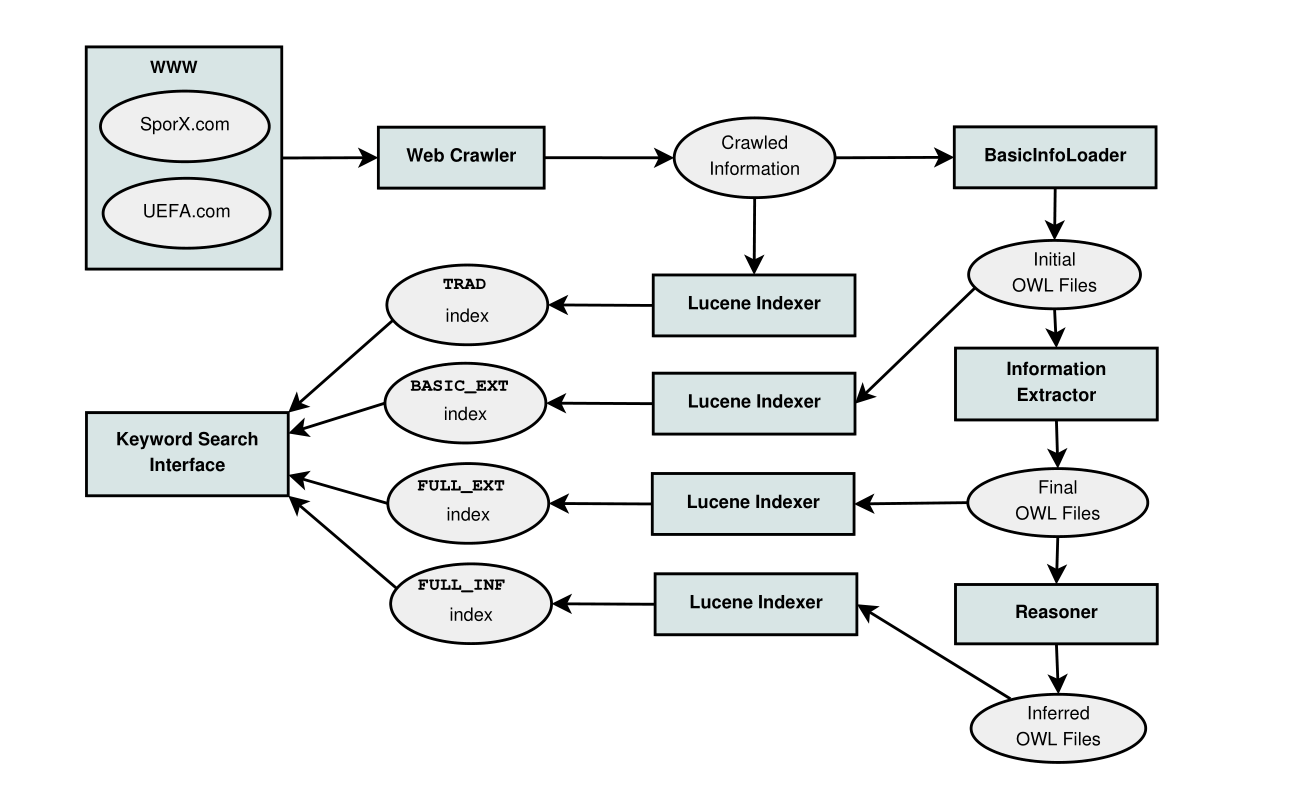
\includegraphics[scale=1.5]{ref_8_design.png}
	\caption{System design of the proposed semantic retrieval system system.}
\end{figure}

\break

So, in this system, information is gathered from \url{www.uefa.com} and \url{www.sporx.com} which
are not semantically readable. These information are then fed into  Lucene Indexer and
owl ontologies are formed from the gathered xml. In this way, both a indexed search engine and semantically 
vaiable Knowledge base is created which are interlinked. Semantic ruleset is created and a 
reasoner is used. So, information can be looked up efficently and accurately.

\section{Reference 10: Towards Efficient SPARQL Query Processing on RDF Data}

In this original research paper, the authors talk about SPARQL query optimiztion. The main claims
of the authors are, in some RDF data storage systems (eg. APACHE Jena, SOR), SPARQL queries are often 
translated into SQL statements. But as SPARQL triples does not translate well enough into SQL statements,
many self-joins and table joins are required which causes slow-downs. \\

To properly index RDF/SQL The authors propose:
\begin{enumerate}
    \item Give each RDF row their own ID. More like whone PostgreSQL stores JSON data 
        like document objects.
        \begin{figure}[h]
        	\label{sparql_id}
        	\centering 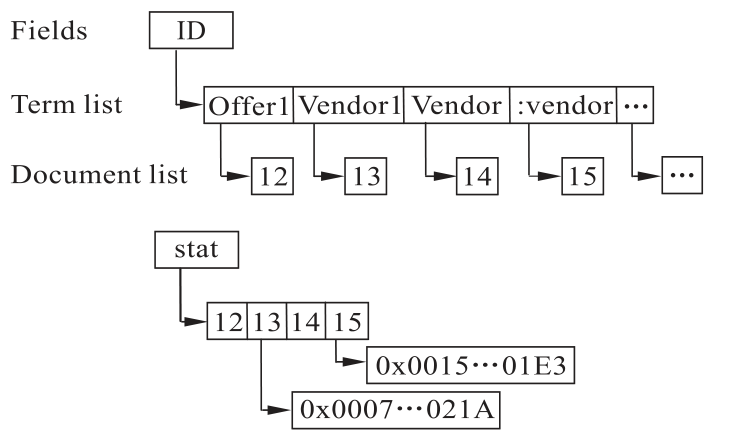
\includegraphics[scale=.35]{sparql_id}
        	\caption{Assigning ID to SPARQL Triples.}
        \end{figure}
    \item Index RDF triple. The authors give some complex schemes.
    \item Optimize query execution and convert SPARQL RDFs into a Tree.
\end{enumerate}



\section{Reference 14: Visualizing search results and document collections using topic maps}

In this descriptive journal paper, the authors discuss how topic maps can be of use on visualizing 
information gathered by conducting search. \\

Also, the authors discuss how to use topic models to mine data for unsupervised learning.
Latent Dirichlet Allocations ie. Topic Maps can create probabilistic models for creating 
classification of text documents.

\break

\section{Reference 15: Topic Map Existing Tools: A Brief Review}

This is also a descriptive article regarding topic maps. Topics include:
\begin{enumerate}
    \item What is a topic map? How are different entities interconnected?
    \item What software to use? How can they be compared?
        \begin{itemize}
            \item XML Topic Maps \cite{XTM}
            \item TOLOG
            \item Topic Map Engines:
                \begin{enumerate}
                    \item GooseWorks
                    \item Omnigator by Ontopia
                    \item SemanText
                    \item empolis k42
                    \item Tm4Jscript
                    \item tmproc
                    \item tinyTIM
                    \item TM4J
                    \item xSiteable
                \end{enumerate}
            \item Topic Map Navigator - Visualizers:
                \begin{enumerate}
                    \item HyperGraph 
                    \item Panckoucke 
                    \item The `V' Topic Map Browser
                    \item ThinkGraph 
                    \item TM3D
                    \item TM4Web/Velocity 
                    \item UNIVIT
                    \item TMNAV
                \end{enumerate}
            \item Topic Map Editors:
                \begin{enumerate}
                    \item AsTMa 
                    \item LTM
                    \item mapalizer
                    \item Simple Topic Maps Management
                    \item Topic Map Designer
                    \item TMTab
                \end{enumerate}
        \end{itemize}
\end{enumerate}


\chapter{Analyis of Citations of Given Paper}

Using google scholar\footnote{\url{scholar.google.com}} I have been able to find two scientific articles that cite 
the given paper as a reference. 

\section{List of Citations}

\begin{enumerate}
	\item Tim Breedveld (July 10, 2018): Finding Similar Software with	Ontology Matching Techniques\
		Master Thesis, Utrecht University
    \item Diana Kocanjer, Nikola Kadoić (April, 18 - 22 2016, GV-Global Virtual Conference):\
    	Raising students awareness about ethical behavior. 
    \item Oscar Karnalim (December 2017): A Low-Level Structure-based Approach for Detecting Source Code Plagiarism.\
    	IAENG International Journal of Computer Science
    \item Claudiu Epure, Adrian Iftene (2016): Analysis of Source Code in Object A Case Study\
        for C\#. Romanian Journal of Human-Computer Interaction 
    \item Feixiang Xu, Xinhui Liu and Chen Zhou (Published: 4 May 2018): Developing an Ontology-Based Rollover\
        Monitoring and Decision Support System for Engineering Vehicles.    
    \item Vilarino Ribeiro, L. (2015). Gestión de Conocimiento en el Diseño\
    	e Implementación de Modelos de Capacidades en Ciencias de la Empresa en escenario EEES.
    \item Xu, Fei-xiang, et al. "An Ontology and AHP Based Quality Evaluation Approach\
    	for Reuse Parts of End-of-Life Construction Machinery." Mathematical Problems in Engineering 2018 (2018).
    \item Wang, Yujun, et al. "Developing an ontology-based cold chain logistics monitoring\
    	and decision system." Journal of Sensors 2015 (2015).
\end{enumerate}

\subsection{Comment}

Citations 6 is written in Spanish and 5, 7-8 are the application of semantic web technologies on
mechanical engineering related topics. We shall discuss citations other than these.

\break

\section{Citation 1: Finding Similar Software with Ontology Matching Techniques}

In this masters thesis, the author tried to implement a prototype for using semantic web 
technologies for software testing. In the end the author created ontologies from source code 
and use semantic matchers to find similiarities between them. The plan is to use these similiarities to
generate automated unit tests. The project is essentially a plagiarism checker for Java. \\

The project works in several layers. The specific matching framework the author is using is 
AgreementMakerLight (AML). 


\begin{figure}[h]
	\label{aml_process}
	\centering 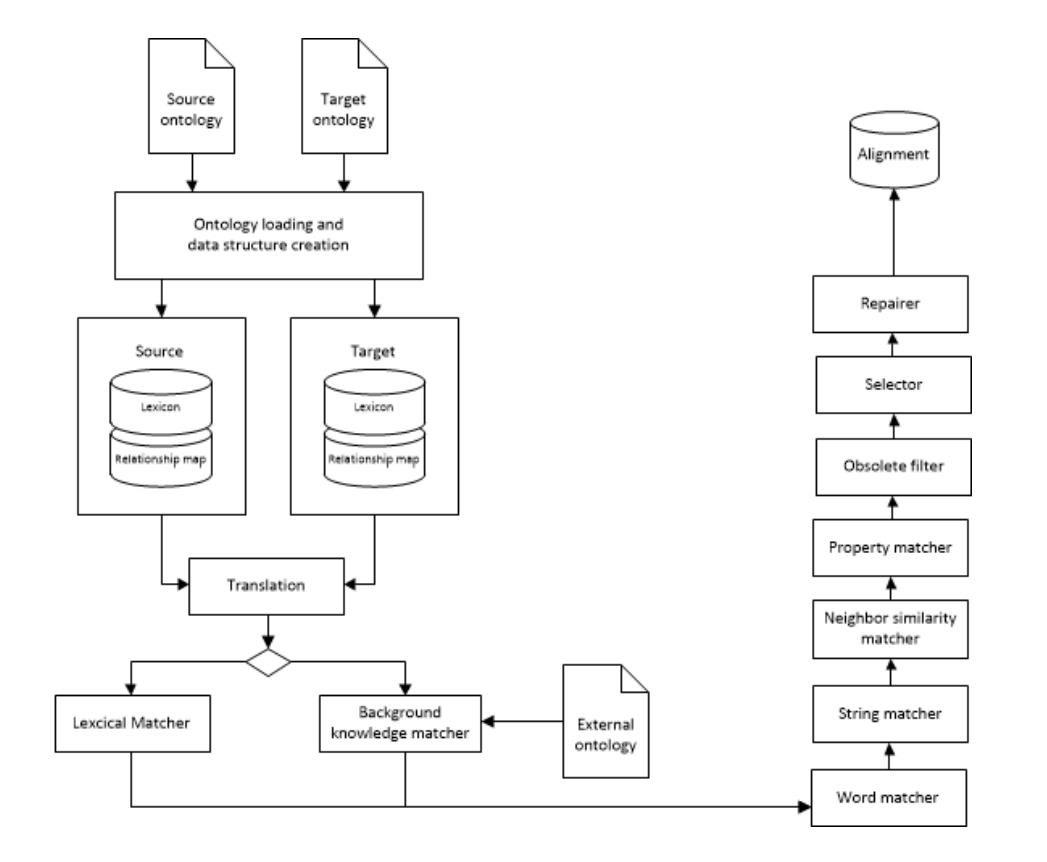
\includegraphics[scale=0.30]{aml_process.png}
	\caption{AML alignment process.}
\end{figure}

So, to align two ontologies, we first extract the ontology from source using Apache Jena
or Spoon. We can extract AST from java classes using these and onwards OWL. After that, 
we insert these both ontologies into AML and it will give a alignment metric.

\section{Citation 2: Raising students awareness about ethical behavior}

This paper is mainly philosophic in nature as it consults with morality and ethics regarding
cheating. Despite conducting surveys the conclusion of the paper is rather subjective as 
the authors link cheating with the culture and economy of their home country of Croatia.

\section{Citation 3: A Low-Level Structure-based Approach for Detecting Source Code Plagiarism}

In this paper, the authors is addressing an important problem of our paper. In our paper,
plagiarism detection is attribute or text based. The author is proposing a Structure-based 
approach. Although the author is calling it 'Low-Level', but actually he is doing a 
java bytecode level comparison already developed by himself in another paper\cite{karnalim2016detecting} \\

\begin{figure}[h]
	\label{low_level_plagiarism_flowchart}
	\centering 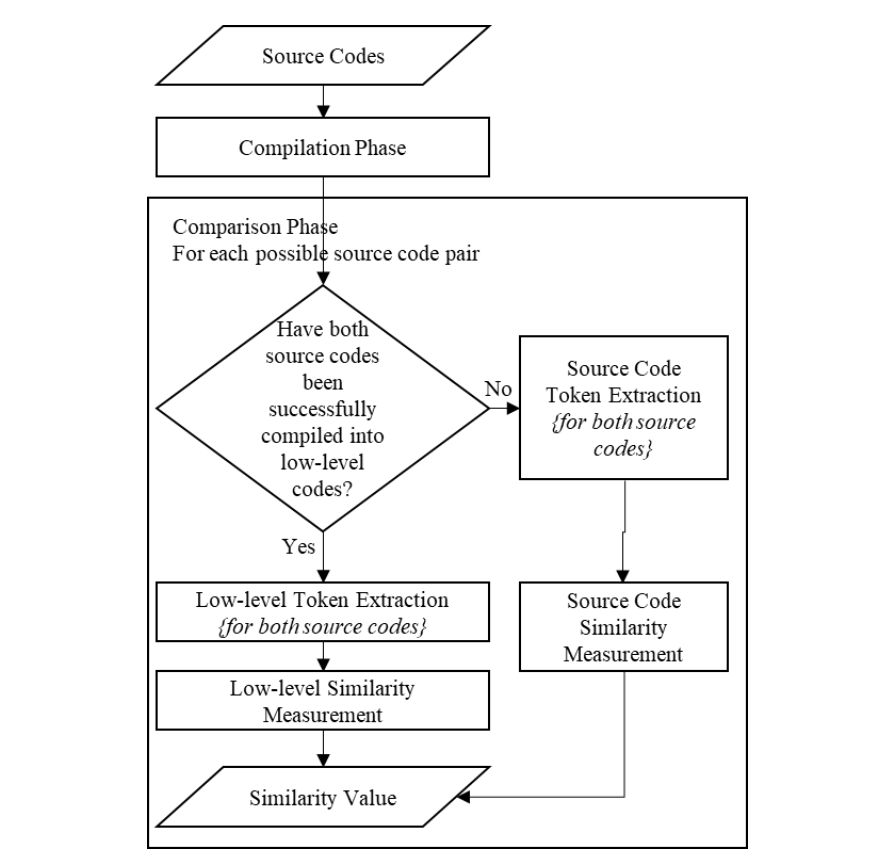
\includegraphics[scale=0.30]{low_level_plagiarism_flowchart.png}
	\caption{Flowchart for "low level" plagiarism detection.}
\end{figure}

From the flow-chart, we can see that there is an extra step of token extraction and token extraction
phase. We also check similiarities between tokens. So it's more like both high-level and low-level
plagiarism detection. \\

\begin{figure}[h]
	\label{low_level_token_extraction}
	\centering 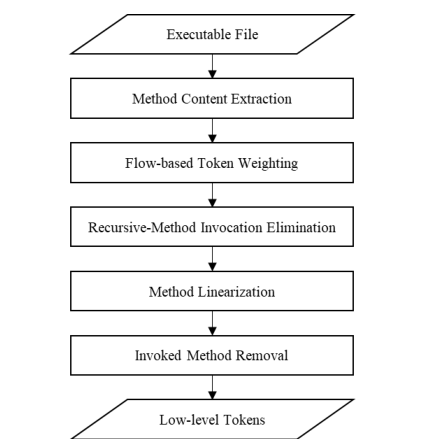
\includegraphics[scale=0.5]{low_level_token_extraction.png}
	\caption{Low level token exraction.}
\end{figure}

Also if we break down the low level token extraction phase, we can see there are several key elements: 
\begin{description}
	\item[Flow-based Token Weighting] There is a flow-based token weighting which depends on basic branch prediction.
		So that unnecessary branching can be ignored.
	\item[Method Content Extraction] It is extracting low level method information from java bytecode.
	\item[Recursive-Method Invocation Elimination] All method calls are converted to directed graoh and 
		we find out strongly connected components and remove them. 
\end{description}

The problem is that, not all programming languages have JIT compilers. A low level language that
compiles directly to machine code or assembly will not be available to be used. High level
languages that uses interpreters will also not be able to use these. LLVM based languages 
or Languages may be able to avail of this offer. \\

\section{Citation 4: Semantic Analysis of Source Code in Object A Case Study for C\#}

This paper is in a unique position as It is similiar to our paper but the authors used an
existing antology (SCRO)\cite{alnusair2012source} and
actually implemented the parser\footnote{\url{https://github.com/mdesalvo/RDFSharp}}. \\

In addition, the authors go several steps ahead of our paper. One is, instead of manually writing 
SPARQL Query, they implement a NLP (Natural Language Processing) toolkit which processes human
readable questions into SPARQL Query.  \\

Another is, instead of storing source code information in OWL or XML/RDF format, the authors have 
created a knowledge base center to host its own triple store for easy information retrieval. \\

And to wrap things up, they have implemented a IIS server with API endpoints to perform query.

\chapter{Future Work}

Extending the future work section discussed in Assignment 1\footnote{\url{https://semantic-web.netlify.com/report/report.pdf}}, we can see that the authors have
specified several further probable developments themselves:

\begin{enumerate}
	\item Create a parser generator so that we can automatically extract ontologies from various sources.
	\begin{itemize}
		\item The authors did not specify any single toolsets for this purpose. I have tried to use:
		\begin{enumerate}
			\item ANTLR for C and Javascript.
			\item Flex/Bison for C.
			\item CodeOntology\footnote{\url{http://codeontology.org/}}\
			\footnote{\url{https://github.com/codeontology/parser}}. of Java. 
		\end{enumerate}
		Although I now think a programming language with static typing like \textit{Haskell} or\
		softly typed like \textit{Typed Racket} would have been better suited.
	\end{itemize}
    \item Create a automated web crawler. It will automatically parse the code and extract the OWL ontology.
    	\begin{itemize}
    		\item Although the authors do no specify anything, the most appropriate place of a crawler\
	    		would be online Disctributed version controlled services. A crawler would run in the servers\
	    		gather semantic information about the source hosted in the server and there should be an\
	    		API endpoints for conducting semantic searches. Semantic information should augment traditional\
	    		indexing based search methods. VCS behemoths like Github\footnote{\url{https://help.github.com/en/articles/navigating-code-on-github}} and Atlassian\
	    		Bitbucket
	    		\footnote{\url{https://bitbucket.org/blog/introducing-code-aware-search-for-bitbucket-cloud}}\
	    		has already started to use semantic technologies to augment the search function.
    		
    		\item Also there are self hosted open source VCSs like Cgit\footnote{\url{https://git.zx2c4.com/cgit/}}\
    			and Gitea\footnote{\url{https://gitea.io/en-us/}} where we can implement our own crawlers.
    	\end{itemize}
    \item Defined metric generator. The program user may define a set of metrics that will\
        be used to measure plagiarism. This set of metrics can be created automatically by using \
        applying Machine Learning or other software development techniques. \\
        This constitutes two things.
        \begin{enumerate}
        	\item Augmenting the parser generator and web crawler so that, it knows which semantic entity to search for\
        		when parsing source code
        	\item Dynamically generate SPARQL query.
        \end{enumerate}
\end{enumerate}

We can extend these goals.

\begin{itemize}
	\item The authors only showed the creation of ontologies from C and Javascript.\
        We can create ontologies from different lanugages from different paradigms. 
    \item The use of \textbf{prolog} to make a better reasoner than reasoners provided by\
    Protege can be done. The application of logic programming will extend the Plagiarism \
    	detectors capabilities. Ontopia omnigator provides a language called tolog\
    	\footnote{\url{https://ontopia.net/omnigator/docs/query/tutorial.html}} for\
    	this specific purpose.
    \item Usage of JSON-LDs. Using JSON datatypes rather than XML/RDF can will greatly extend
    	the capability of our application's interface with modern API paradigms like GraphQL.
\end{itemize}

Doing the above things will allow us to create a automated plagiarism checker which can instantanously
tell us while we are writing code the related source files. So, it shall not only be used for plagiarism detection
but also for intelligent and dynamic code search. 


%%%%%%%%%%%%%%%%%%%%
% Bibilography
%%%%%%%%%%%%%%%%%%%%

\bibliography{citations}{}
\bibliographystyle{plain}


\end{document}
